% === Cours de Java
% === Version couleur pour la présentation

\documentclass[14pt,xcolor,table]{beamer}
\usetheme{Warsaw}

\usepackage{mic}

\title{Microprocesseurs (MIC)}
\subtitle{Chapitre 1 : Ouvrons un PC}
\date{} 

% =====================   DOCUMENT ===================++
\begin{document}

% ---------------------   FRAME   --------------------
\begin{frame}
	\titlepage
\end{frame}

% ---------------------   FRAME   --------------------
\begin{frame}[fragile]{Carte mère}
% ----------------------------------------------------
	
	La \emph{carte mère} (\textit{motherboard})
	permet l'interconnexion des composants d'un ordinateur.
	
	\begin{center}
	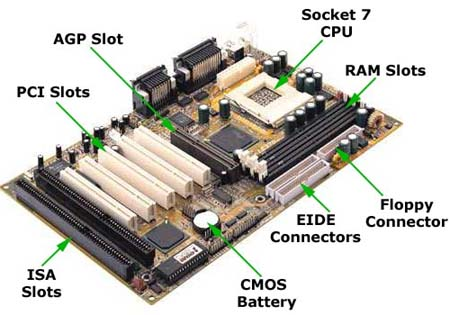
\includegraphics[width=.7\textwidth]{images/motherboard}
	\source{\url{https://ist94.wikispaces.com/file/view/motherboard.jpg/30963019/motherboard.jpg}}
	\end{center}
	
\end{frame}

% ---------------------   FRAME   --------------------
\begin{frame}[fragile]{Carte mère}
% ----------------------------------------------------
	
	\begin{center}
	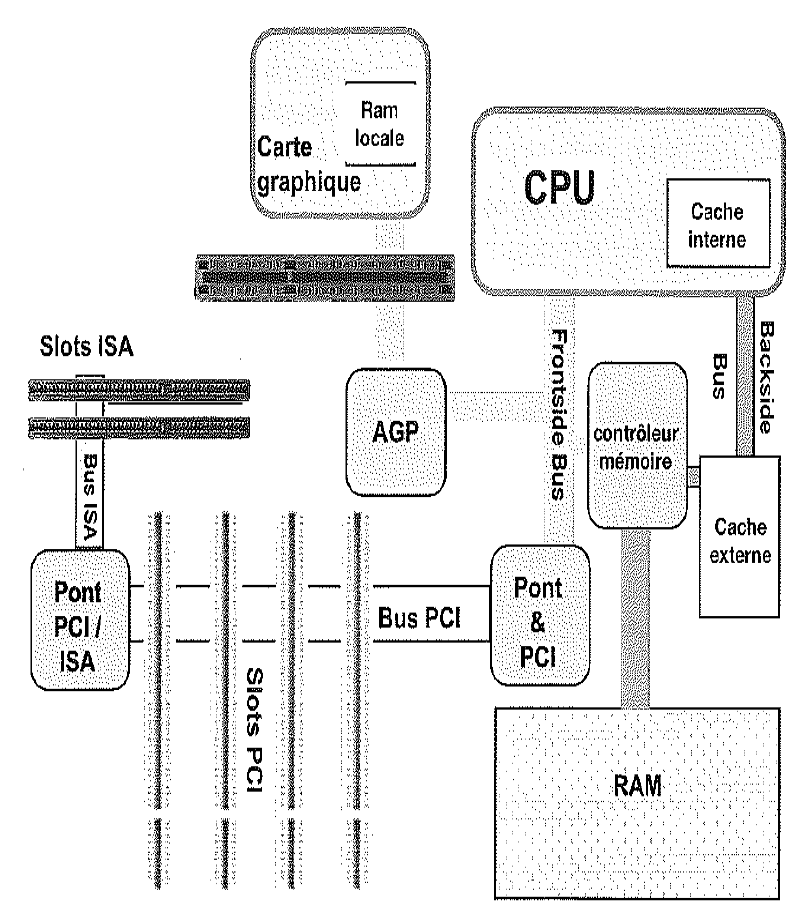
\includegraphics[height=7cm]{images/motherboard-schema}
	\source{inconnue}
	\end{center}
	
\end{frame}

% ---------------------   FRAME   --------------------
\begin{frame}[fragile]{Processeur}
% ----------------------------------------------------
	
	Le \emph{processeur} exécute les programmes
	
	%\begin{center}
	%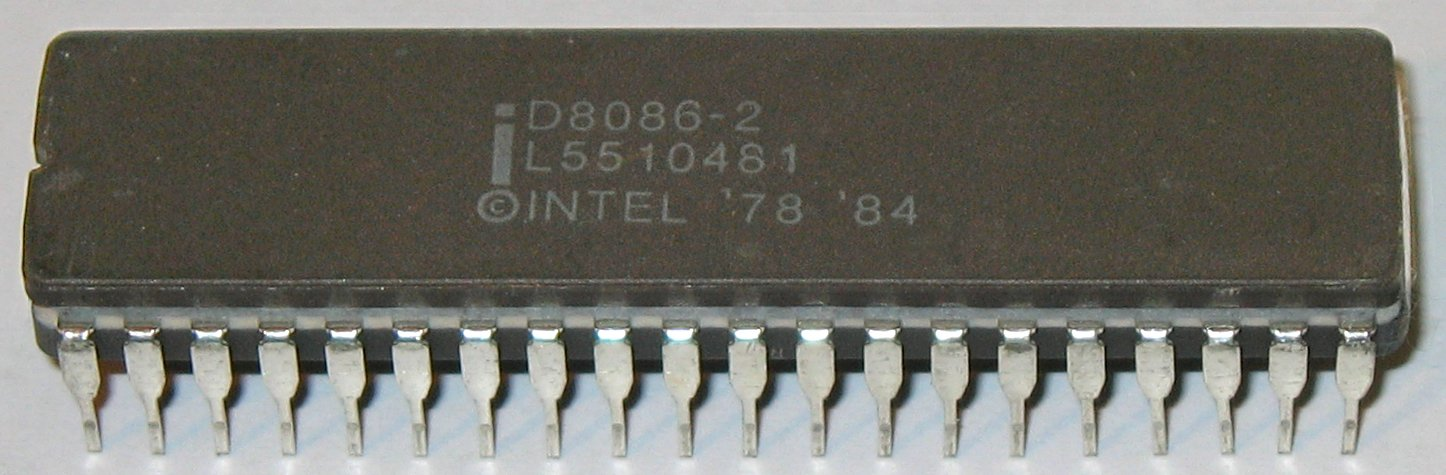
\includegraphics[width=.5\textwidth]{images/cpu-8086}
	%\source{\url{http://upload.wikimedia.org/wikipedia/commons/2/2d/I8086.jpg}}
	%\end{center}

	\begin{center}
	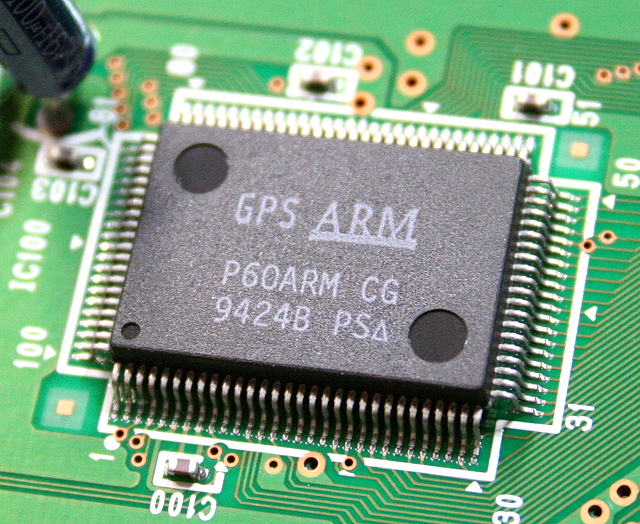
\includegraphics[width=.4\textwidth]{images/cpu-arm60}
	\source{\url{http://fr.wikipedia.org/wiki/Microprocesseur}}
	\end{center}
	
	Un \emph{microprocesseur} est un processeur dont tous les
	composants sont regroupés dans un même boitier
	
\end{frame}

% ---------------------   FRAME   --------------------
\begin{frame}[fragile]{Processeur}
% ----------------------------------------------------
	
	Il communique avec les autres composants via ses \emph{pattes} (\textit{pins})
	
	\bigskip
	
	\begin{tabular}{p{4cm}p{6cm}}
	\begin{minipage}[c]{4cm}
	\begin{center}
	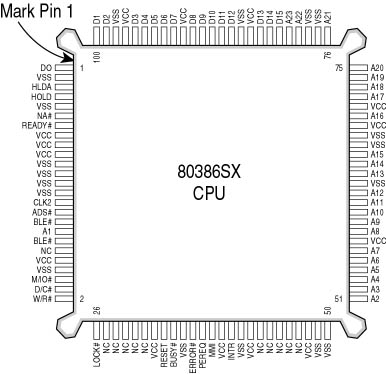
\includegraphics[width=1.1\textwidth]{images/i386-sx}
	\source{inconnue}
	\end{center}
	\end{minipage}
	&
	\begin{minipage}[c]{7cm}
	\small
	\begin{description}
	\item[Di] reliées au bus de données
	\item[Ai] reliées au bus d'adresses
	\item[INTR] pour les interruptions
	\item[CLK] horloge
	\item[RESET] reset du processeur
	\item[Vcc Vss] alimentation
	\item[\dots]
	\end{description}
	\end{minipage}
	\\
	\end{tabular}
	
\end{frame}

% ---------------------   FRAME   --------------------
\begin{frame}[fragile]{Processeur}
% ----------------------------------------------------
	
	Les processeurs se distinguent par
	
	\begin{itemize}
	\item leur architecture interne
	\item les instructions comprises
	\item la taille des registres (32/64 bits)
	\item leur fréquence
	\item le nombre de \textit{c\oe{}urs}
	\item \dots
	\end{itemize}
	
\end{frame}

% ---------------------   FRAME   --------------------
\begin{frame}[fragile]{Famille de processeurs}
% ----------------------------------------------------
	
	Une \emph{famille} de processeurs regroupe
	les processeurs qui partagent un même jeu
	d'instructions.

	\bigskip
	Quelques dates de la famille \emph{x86}
	\begin{description}
	\item[1978] Intel 8086
	\item[1985] Intel 80386, AMD Am386
	\item[1993] Intel Pentium (Pro)
	\item[2000] Intel Pentium 4, Athlon
	\item[2008] Intel Core i7
	\item[\dots]
	\end{description}
	
\end{frame}

% ---------------------   FRAME   --------------------
\begin{frame}[fragile]{RISC vs CISC}
% ----------------------------------------------------

On distingue également les processeurs de type \emph{RISC} et \emph{CISC}

\bigskip
\begin{footnotesize}
\begin{tabular}{rp{3cm}p{3cm}}
	& \emph{RISC} & \emph{CISC} \\\hline
Signification & Reduced Instruction Set Computer & Complex Instruction Set Computer \\\hline
Nb d'instructions & Plus & Moins \\\hline
Code & Plus gros & Moins gros \\\hline
Processeur & Moins complexe & Plus complexe \\\hline
\end{tabular}
\end{footnotesize}

\bigskip
Les \emph{x86} sont des \emph{CISC}

\end{frame}

% ---------------------   FRAME   --------------------
\begin{frame}[fragile]{La mémoire}
% ----------------------------------------------------
	
	La \emph{RAM} est la mémoire vive qui contient les
	processus (code + données)

	\begin{center}
	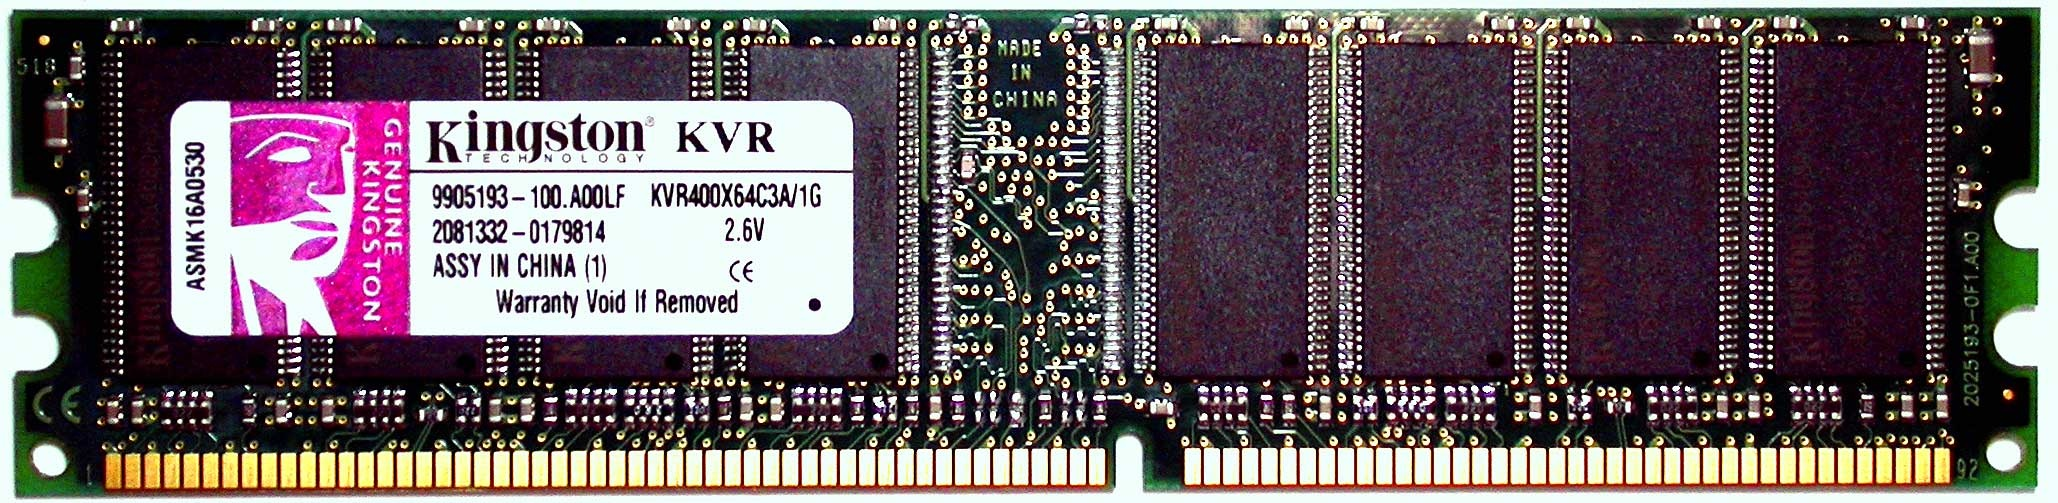
\includegraphics[width=.7\textwidth]{images/ram-barette}
	\source{\url{http://upload.wikimedia.org/wikipedia/commons/1/18/DDRSDRAM400-1GB.jpg}}
	\end{center}
	
	\begin{itemize}
	\item Différentes technologies
	\item Utilisation de caches (L1, L2, L3)
	\end{itemize}
	
\end{frame}

% ---------------------   FRAME   --------------------
\begin{frame}[fragile]{La mémoire}
% ----------------------------------------------------
	
	\begin{center}
	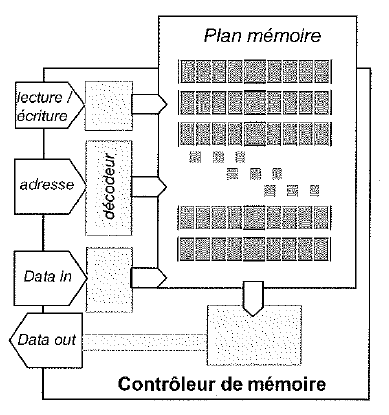
\includegraphics[width=.6\textwidth]{images/RAM}
	\source{inconnue}
	\end{center}
	
\end{frame}



% ------------------------------------------------------
\end{document}
